\documentclass[aspectratio=169,11pt]{beamer}

\usepackage{graphicx}
\usepackage{tikz}
\usetikzlibrary{positioning,arrows.meta}
\usepackage{xcolor}
\usepackage{booktabs}
\usepackage{tabularx}
\usepackage{array}
\usepackage{ragged2e}

\definecolor{GEUBlue}{RGB}{20,55,105}
\definecolor{GEULightBlue}{RGB}{238,244,251}
\definecolor{GEUGrey}{RGB}{90,90,90}
\definecolor{GEULightGrey}{RGB}{245,246,248}

\usetheme{default}
\setbeamertemplate{navigation symbols}{}
\setbeamertemplate{blocks}[rounded][shadow=false]
\setbeamercolor{normal text}{fg=black,bg=white}
\setbeamercolor{frametitle}{fg=GEUBlue}
\setbeamercolor{structure}{fg=GEUBlue}
\setbeamercolor{block title}{fg=GEUBlue,bg=GEULightBlue}
\setbeamercolor{block body}{fg=black,bg=GEULightBlue}
\setbeamerfont{frametitle}{size=\Large,series=\bfseries}

% Replace with the actual logo filename
\newcommand{\GEULogo}{graphicera_logo.png}

% Header and footer
\setbeamertemplate{headline}{%
  \begin{tikzpicture}[remember picture,overlay]
    \node[anchor=north east,xshift=-0.30cm,yshift=-0.12cm]
      at (current page.north east)
      {\includegraphics[height=0.62cm]{\GEULogo}};
  \end{tikzpicture}
  \vspace{0.72cm}
}
\setbeamertemplate{frametitle}{%
  \vspace{0.03cm}
  \insertframetitle\par
  \vspace{0.04cm}
  \textcolor{GEUBlue}{\rule{\textwidth}{0.9pt}}
  \vspace{0.03cm}
}
\setbeamertemplate{footline}{%
  \leavevmode
  \hbox{%
  \begin{beamercolorbox}[wd=.82\paperwidth,ht=0.32cm,dp=0.10cm,leftskip=.3cm]{author in head/foot}
    \tiny Department of Computer Science \& Engineering | Graphic Era (Deemed to be University)
  \end{beamercolorbox}%
  \begin{beamercolorbox}[wd=.18\paperwidth,ht=0.32cm,dp=0.10cm,rightskip=.3cm]{date in head/foot}
    \hfill\tiny\insertframenumber/\inserttotalframenumber
  \end{beamercolorbox}}
}

\newcommand{\smallnote}[1]{\vspace{0.08cm}{\scriptsize\color{GEUGrey}#1}}
\newcommand{\placeholder}[1]{\textit{\color{GEUGrey}#1}}

\title{\textbf{Project-Based Learning}\\[2mm]\large Phase-I Evaluation}
\author{\textbf{Smart Driver Drowsiness \& Safety System}\\Team ID: DSCPP-III-2026-T234}
\institute{Department of Computer Science \& Engineering\\Graphic Era (Deemed to be University), Dehradun}
\date{Academic Session 2026--27}

\begin{document}

% 1
\begin{frame}[plain]
\begin{tikzpicture}[remember picture,overlay]
\draw[GEUBlue,line width=3pt] (current page.north west) -- (current page.north east);
\node[anchor=north east,xshift=-0.45cm,yshift=-0.35cm] at (current page.north east)
{\includegraphics[height=1.0cm]{\GEULogo}};
\node[align=center,text width=.84\paperwidth] at ([yshift=.25cm]current page.center)
{{\color{GEUBlue}\fontsize{26}{30}\selectfont\bfseries PROJECT-BASED LEARNING}\\[3mm]
 {\fontsize{18}{22}\selectfont PHASE-I EVALUATION}\\[7mm]
 {\color{GEUGrey}\Large\bfseries \placeholder{Smart Driver Drowsiness \& Safety System}}\\[3mm]
 {\color{GEUBlue}\normalsize Team ID: DSCPP-III-2026-T234}};
\node[align=center,anchor=south,yshift=.42cm] at (current page.south)
{\bfseries Department of Computer Science \& Engineering\\
Graphic Era (Deemed to be University), Dehradun\\[-1mm]
\scriptsize Academic Session 2026--27};
\end{tikzpicture}
\end{frame}

% 2
\begin{frame}{Team \& Mentor Details}
\begin{columns}[T,totalwidth=\textwidth]
\column{.48\textwidth}
\begin{block}{Team Information}
\begin{tabular}{@{}ll@{}}
\textbf{Team ID:} & DSCPP-III-2026-T234\\
\textbf{Semester:} & 3rd\\
\textbf{Section:} & H / E / ML4 / ML3\\
\textbf{Domain:} & \placeholder{C++ \& Computer Vision}
\end{tabular}
\end{block}
\column{.48\textwidth}
\begin{block}{Team Members}
1.\quad \placeholder{RIDVIK GARG -- 2028039}\\
2.\quad \placeholder{Prabhav Gulyani -- 2027975}\\
3.\quad \placeholder{Nandini Gupta -- 2028777}\\
4.\quad \placeholder{Antriksh Gehlot -- 2028648}
\end{block}
\end{columns}
\vspace{2mm}
\begin{block}{Mentor}
\placeholder{Mr. Kamal Kumar Gola}
\hfill
\textbf{Interactions completed: 3} 
\end{block}
\end{frame}

% 3 
\begin{frame}{Problem Statement \& Motivation}
\begin{block}{Problem Statement}
\placeholder{If a driver gets tired, they can lose attention on the road, especially on long night trips. Many existing student projects only check for closed eyes and just give a basic beep sound, which is not enough.}
\end{block}
\vspace{-3mm}
\begin{columns}[T,totalwidth=\textwidth]
\column{.48\textwidth}
\textbf{\color{GEUBlue}Motivation}
\vspace{-1mm}
\begin{itemize}\itemsep0pt
\item \placeholder{To stop accidents that happen when drivers fall asleep.}
\item \placeholder{Current small projects don't check distraction and sleepiness together.}
\item \placeholder{Just an alarm is not enough; we need music control and SMS alerts.}
\end{itemize}
\column{.48\textwidth}
\textbf{\color{GEUBlue}Target Users / Stakeholders}
\vspace{-1mm}
\begin{itemize}\itemsep0pt
\item \placeholder{People driving at night or on long journeys.}
\item \placeholder{Family members who want to ensure the driver's safety.}
\item \placeholder{General road safety for everyone.}
\end{itemize}
\end{columns}
\end{frame}

% 4
\begin{frame}{Objectives}
\textbf{\color{GEUBlue}Project Objectives}
\vspace{2mm}
\begin{enumerate}\itemsep5pt
\item \placeholder{Check if the driver's eyes stay closed for too long.}
\item \placeholder{Find out if the driver is looking away from the road (distraction).}
\item \placeholder{Give a normal warning first, and a loud alarm if they ignore it.}
\item \placeholder{Pause or lower the car's music volume during the warning.}
\item \placeholder{Send a text message to a saved family contact in critical cases.}
\end{enumerate}
\vfill
\begin{center}
\colorbox{GEULightBlue}{\parbox{.80\textwidth}{\centering
\textbf{Key Objective:} \placeholder{To build a working safety prototype that monitors the driver, warns them, controls music, and saves the events.}}}
\end{center}
\end{frame}

% 5
\begin{frame}{Proposed Solution}
\begin{columns}[T,totalwidth=\textwidth]
\column{.48\textwidth}
\textbf{\color{GEUBlue}Proposed Approach}
\begin{enumerate}\itemsep1pt
\item \placeholder{Input: Camera captures the driver's video feed.}
\item \placeholder{Processing: OpenCV checks the face and eyes.}
\item \placeholder{System Logic: C++ code decides if the driver is sleepy.}
\item \placeholder{Database: SQLite saves the history of warnings.}
\item \placeholder{Output: Speaker alarm, music control, and family SMS.}
\end{enumerate}
\column{.48\textwidth}
\textbf{\color{GEUBlue}Key Features}
\begin{itemize}\itemsep1pt
\item \placeholder{Checks both sleepiness and looking away.}
\item \placeholder{Automatically stops or lowers the music.}
\item \placeholder{Emergency message feature for family.}
\item \placeholder{Shows live status (Good, Warning, Critical).}
\item \placeholder{Uses Linked List, Queue, and Stack for data.}
\end{itemize}
\end{columns}
\vfill
\smallnote{Instead of just sounding an alarm, our system lowers the music so the driver can actually hear the warning.}
\end{frame}

% 6
\begin{frame}{Integration of PBL Course Concepts}
\scriptsize
\begin{center}
\renewcommand{\arraystretch}{1.25}
\begin{tabularx}{.96\textwidth}{@{}>{\bfseries}p{3.0cm}X p{2.5cm}@{}}
\toprule
Course & Concepts Applied & Project Module\\
\midrule
Data Structures in C & \placeholder{Linked List (history), Queue (events), Stack (recent alerts)} & \placeholder{Event Manager}\\
OOPs with C++ & \placeholder{C++ classes, objects, and OpenCV functions} & \placeholder{Core Logic}\\


\bottomrule
\end{tabularx}
\end{center}
\vfill
\begin{center}
\colorbox{GEULightBlue}{\parbox{.86\textwidth}{\centering
\textbf{Requirement:} Demonstrate meaningful integration of both subjects in \textbf{one} project.}}
\end{center}
\end{frame}

% 7
\begin{frame}{System Architecture / Workflow}
\begin{center}
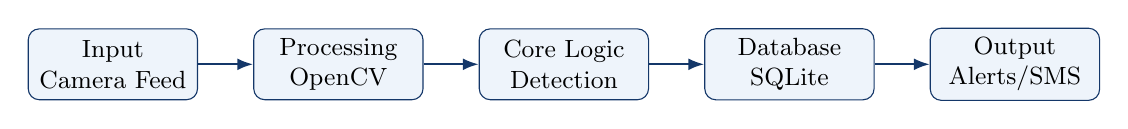
\begin{tikzpicture}[
node distance=7mm,
box/.style={rectangle,rounded corners,draw=GEUBlue,fill=GEULightBlue,
minimum width=2.15cm,minimum height=9mm,align=center,font=\small},
arrow/.style={-{Latex[length=2mm]},thick,draw=GEUBlue}
]
\node[box] (a) {Input\\Camera Feed};
\node[box,right=of a] (b) {Processing\\OpenCV};
\node[box,right=of b] (c) {Core Logic\\Detection};
\node[box,right=of c] (d) {Database\\SQLite};
\node[box,right=of d] (e) {Output\\Alerts/SMS};
\draw[arrow] (a)--(b); \draw[arrow] (b)--(c); \draw[arrow] (c)--(d); \draw[arrow] (d)--(e);
\end{tikzpicture}
\end{center}
\vspace{3mm}
\begin{columns}[T,totalwidth=\textwidth]
\column{.48\textwidth}
\textbf{\color{GEUBlue}Major Components}
\begin{itemize}\itemsep0pt
\item \placeholder{Camera input module}
\item \placeholder{Face and eye tracking logic}
\item \placeholder{Alert and Event handling system}
\end{itemize}
\column{.48\textwidth}
\textbf{\color{GEUBlue}Data / Control Flow}
\begin{itemize}\itemsep0pt
\item \placeholder{Camera sends frames to OpenCV.}
\item \placeholder{Code checks for closed eyes or distraction.}
\item \placeholder{If unsafe, it triggers alarm, stops music, saves event.}
\end{itemize}
\end{columns}
\end{frame}

% 8
\begin{frame}{Technology Stack \& Methodology}
\begin{columns}[T,totalwidth=\textwidth]
\column{.48\textwidth}
\begin{block}{Technology Stack}
\begin{itemize}\itemsep1pt
\item Programming: \placeholder{C++}
\item Database: \placeholder{SQLite}
\item Tools / Framework: \placeholder{OpenCV}
\item IDE: \placeholder{VS Code}
\item Version Control: \placeholder{Git / GitHub}
\end{itemize}
\end{block}
\column{.48\textwidth}
\begin{block}{Development Methodology}
\begin{enumerate}\itemsep1pt
\item \placeholder{Understand requirements and plan modules}
\item \placeholder{Write code for OpenCV face detection}
\item \placeholder{Add logic for alerts and music control}
\item \placeholder{Connect SQLite DB and Data Structures}
\item \placeholder{Final testing and bug fixing}
\end{enumerate}
\end{block}
\end{columns}
\vfill
\begin{center}
\smallnote{We chose C++ and OpenCV because they are fast and good for real-time video processing.}
\end{center}
\end{frame}

% 9
\begin{frame}{Initial Progress \& Team Contribution}
\begin{columns}[T,totalwidth=\textwidth]
\column{.44\textwidth}
\textbf{\color{GEUBlue}Progress Achieved}
\begin{itemize}\itemsep1pt
\item \placeholder{Decided project requirements and modules}
\item \placeholder{Designed the basic system architecture}
\item \placeholder{Planned how to use Queue, Stack, and Linked List}
\item \placeholder{Created the SQLite database tables}
\item \placeholder{Tested basic camera input with OpenCV}
\end{itemize}
\column{.52\textwidth}
\textbf{\color{GEUBlue}Individual Contribution}
\vspace{2mm}
\scriptsize
\begin{tabularx}{\textwidth}{@{}p{1.8cm}p{2.0cm}X@{}}
\toprule
Member & Role & Contribution\\
\midrule
\placeholder{RIDVIK} & \placeholder{Team Lead} & \placeholder{Core Logic \& Architecture}\\
\placeholder{Prabhav} & \placeholder{Developer} & \placeholder{OpenCV Drowsiness Code}\\
\placeholder{Nandini} & \placeholder{DB/Testing} & \placeholder{SQLite \& Distraction Code}\\
\placeholder{Antriksh} & \placeholder{Developer} & \placeholder{Music Control \& Alerts}\\
\bottomrule
\end{tabularx}
\end{columns}
\end{frame}

% 10 
\begin{frame}{Roadmap, Expected Outcomes \& References}
\vspace{-3mm}
\begin{columns}[T,totalwidth=\textwidth]
\column{.47\textwidth}
\textbf{\color{GEUBlue}Roadmap}
\vspace{-1mm}
\begin{enumerate}\itemsep0pt
\item \placeholder{Phase-I: Project planning and basic design}
\item \placeholder{Phase-II: Writing OpenCV and Database code}
\item \placeholder{Phase-III: Joining all parts and final testing}
\end{enumerate}
\vspace{2mm}
\textbf{\color{GEUBlue}Expected Outcomes}
\vspace{-1mm}
\begin{itemize}\itemsep0pt
\item \placeholder{A working prototype for driver safety}
\item \placeholder{Working music control and SMS alert feature}
\item \placeholder{Live display showing Good, Warning, or Critical}
\item \placeholder{Project source code and final report}
\end{itemize}
\column{.47\textwidth}
\textbf{\color{GEUBlue}References}
\vspace{-1mm}
\begin{enumerate}\itemsep0pt
\item \placeholder{OpenCV Documentation Computer Vision Library}
\item \placeholder{SQLite Documentation Lightweight Database Engine}
\item \placeholder{C++ Reference Standard C++ Language and Library}
\item \placeholder{OS concepts related to threads and synchronization}
\end{enumerate}
\vspace{4mm}
\begin{center}
\colorbox{GEUBlue}{\parbox{.78\textwidth}{\centering\color{white}\textbf{Thank You}\\Questions \& Suggestions}}
\end{center}
\end{columns}
\end{frame}

\end{document}